\documentclass[conference,10pt]{IEEEtran}
\usepackage{cite,amsmath,amssymb,amsfonts,graphicx,textcomp,xcolor,hyperref,booktabs,multirow,enumitem,balance}
\usepackage{tikz,pgfplots}
\pgfplotsset{compat=1.17}
\usetikzlibrary{shapes.geometric,arrows.meta,positioning,calc}
\usepackage{listings}
\usepackage{stfloats}
\lstset{basicstyle=\ttfamily\scriptsize,breaklines=true,frame=single,backgroundcolor=\color{gray!5}}
\setlist{nosep,leftmargin=*}
\renewcommand{\topfraction}{0.95}
\renewcommand{\bottomfraction}{0.95}
\renewcommand{\textfraction}{0.05}
\renewcommand{\floatpagefraction}{0.85}
\setcounter{topnumber}{8}
\setcounter{bottomnumber}{8}
\setcounter{totalnumber}{16}
\setcounter{dbltopnumber}{4}
\definecolor{nv}{RGB}{118,185,0}
\definecolor{am}{RGB}{200,40,40}
\definecolor{il}{RGB}{0,113,197}
\definecolor{gc}{RGB}{66,133,244}
\definecolor{t1}{RGB}{41,128,185}
\definecolor{t2}{RGB}{142,68,173}
\definecolor{t3}{RGB}{211,84,0}
\definecolor{t4}{RGB}{192,57,43}

\begin{document}
\title{OpenDeepBench and OpenDeepAPM: Deep Infrastructure\\Benchmarking and Trace-Correlated Observability\\for Multi-Cloud LLM Inference}
\author{
\IEEEauthorblockN{Srikanta Datta Tumkur\IEEEauthorrefmark{1}, Anshu Bansal\IEEEauthorrefmark{1}, Mehar Simhadri\IEEEauthorrefmark{2}, Jay Iyer\IEEEauthorrefmark{2}}
\IEEEauthorblockA{\IEEEauthorrefmark{1}MIT Sloan School of Management, Cambridge, MA -- \texttt{\{srikanta, anshu.bansal\}@sloan.mit.edu}}
\IEEEauthorblockA{\IEEEauthorrefmark{2}IEEE Senior Members -- \texttt{\{meher.simhadri, jay.iyer\}@ieee.org}}
}
\maketitle

\begin{abstract}
Large Language Model (LLM) inference has evolved from single-GPU prototypes into production-grade, multi-cloud infrastructure spanning heterogeneous accelerator architectures. Yet the benchmarking and observability ecosystems remain critically fragmented: MLPerf Inference measures raw throughput on fixed models in single-cloud settings; traditional APM tools designed for deterministic microservices fail catastrophically for non-deterministic LLM inference; and no platform today provides end-to-end trace correlation from user traffic through GPU silicon to root cause. We present two complementary systems. \textbf{OpenDeepAPM} is a deep LLM Application Performance Monitoring architecture that constructs unified traces spanning 27 linked spans across seven layers---from client traffic and CPU preprocessing through GPU prefill/decode phases, per-rank tensor-parallel execution, per-layer attention and MLP operations, NCCL/NVLink/InfiniBand collectives, KV-cache lifecycle, and storage---with silicon metrics (SM utilization, tensor core activity, HBM bandwidth, L2 hit rates) attached as evidence to each span via NVTX-linked CUDA timelines and DCGM counters. The correlation engine joins traces using composite keys (trace\_id + time\_window + node\_id + gpu\_uuid + rank\_id + nccl\_comm\_id + nic\_id) across a time-series graph database to produce automated root-cause attribution. \textbf{OpenDeepBench} is a multi-cloud, multi-silicon, multi-model LLM infrastructure benchmark that evaluates 16 dimensions---cloud provider, region, silicon vendor, accelerator model, serving engine, runtime, collective backend, model size, context size (1K--128K), output length, concurrency, batch policy, KV-cache mode, attention type, network topology, and storage---producing a normalized scorecard of TTFT, TPOT, throughput, cost/token, energy/token, and reliability with automated root-cause diagnosis. Across 11 cloud providers, 6 accelerator families, and 12 benchmark suites (ODB-Chat through ODB-Reliability), OpenDeepBench reveals: (1)~3.2$\times$ throughput variance for identical models across clouds; (2)~KV-cache memory bandwidth as the dominant decode bottleneck with TPOT degrading sharply beyond 32K context; (3)~AMD MI355X achieving 97\% of NVIDIA B200 decode performance at 35\% lower cost; (4)~inter-node fabric congestion as the primary source of p99 latency spikes in multi-node tensor-parallel deployments; and (5)~cross-cloud disaggregated inference reducing cost 15--29\% at iso-latency. We detail the OpenTelemetry integration architecture, time-series graph correlation engine, compliance framework, and propose the OpenDeepBench Composite Score as a new industry standard.
\end{abstract}
\begin{IEEEkeywords}
LLM inference, deep APM, distributed tracing, OpenTelemetry, multi-cloud benchmarking, GPU observability, KV-cache, NCCL, NVLink, InfiniBand, root-cause analysis, time-series graph database
\end{IEEEkeywords}

%===================================================================
\section{Introduction}
%===================================================================
The AI inference landscape has entered a new era. Global spending on AI infrastructure exceeded \$200B in 2025, yet organizations deploying LLMs in production face a dual paradox: the benchmarks used to select hardware measure almost none of the metrics that determine real-world performance, and the monitoring tools used to operate inference infrastructure were designed for a fundamentally different class of workloads.

\textbf{Gap 1: The Benchmark-Production Disconnect.} MLPerf Inference v6.0~\cite{mlcommons2026mlperfv6} evaluates raw throughput on fixed models in controlled, single-cloud environments. Production inference deployments include guardrails~\cite{inan2023llamaguard}, PII masking, watermarking~\cite{kirchner2024watermarking}, and compliance logging that add 18--61\% latency. No existing benchmark answers: ``Which cloud + GPU + serving engine + context size gives the best TTFT, TPOT, throughput, cost/token, and reliability under realistic multi-tenant traffic?''

\textbf{Gap 2: The Observability Void.} Traditional APM tools (Datadog, New Relic, Dynatrace) instrument deterministic microservices with request-response spans. LLM inference is fundamentally different: a single request generates a \emph{trace} containing dozens of linked spans across traffic ingress, CPU tokenization, GPU scheduling, tensor-parallel prefill across 16 ranks on 2 nodes, 80 transformer layers per phase, NCCL collectives over NVLink and InfiniBand, paged KV-cache allocation and lifecycle, autoregressive decode with growing context, and response streaming. No existing platform correlates GPU thermal throttling with output quality degradation, or KV-cache eviction with downstream accuracy loss, or NCCL stalls with per-token latency spikes.

\textbf{Gap 3: Architecture Blind Spots.} NVIDIA-centric benchmarks systematically favor compute-bound workloads. AMD Instinct MI355X~\cite{amd2025mi350} with 288\,GB HBM3E and Intel Gaudi~3~\cite{intel2025gaudi3} with cost-optimized matrix engines excel in memory-bound and energy-constrained regimes that current benchmarks underrepresent.

This paper addresses all three gaps through two complementary systems:

\textbf{OpenDeepAPM} provides deep, end-to-end trace correlation for LLM inference. Unlike traditional APM that generates one span per service call, OpenDeepAPM constructs traces with 27+ linked spans covering every layer from client traffic to GPU silicon. The correlation engine joins OpenTelemetry traces, NVTX-linked CUDA timelines, DCGM/rocm-smi hardware counters, NCCL communication logs, NVLink/InfiniBand fabric telemetry, and storage metrics into a unified time-series graph database for automated root-cause attribution.

\textbf{OpenDeepBench} provides deep, multi-dimensional LLM infrastructure benchmarking. Unlike MLPerf (which answers ``which GPU is faster?'') or vLLM benchmarks (which measure runtime throughput), OpenDeepBench answers: ``For this model, at this context size, on this cloud, on this silicon, with this serving engine and this traffic pattern---what is the TTFT, TPOT, throughput, cost/token, and \emph{why}?''

\subsection{Contributions}
\begin{enumerate}
\item \textbf{OpenDeepAPM}: A 27-span, 7-layer deep trace architecture for LLM inference with composite join keys linking request causality to GPU silicon evidence (Section~\ref{sec:deepapm}).
\item \textbf{Correlation engine}: A time-series graph database architecture joining OpenTelemetry traces, NVTX timelines, DCGM counters, NCCL logs, and fabric telemetry for automated root-cause diagnosis (Section~\ref{sec:correlation}).
\item \textbf{OpenDeepBench}: A 16-dimension, 12-suite benchmark framework for multi-cloud, multi-silicon LLM infrastructure with normalized scorecards (Section~\ref{sec:deepbench}).
\item \textbf{Multi-silicon normalization}: Architecture-neutral evaluation across NVIDIA, AMD, Intel, and Google accelerators with unified semantic conventions (Section~\ref{sec:arch}).
\item \textbf{Root-cause diagnosis}: Four validated case studies demonstrating automated attribution across KV-cache, network, traffic, and storage bottlenecks (Section~\ref{sec:rootcause}).
\item \textbf{OpenDeepBench Composite Score}: A weighted scoring model with 12 benchmark suite categories from production operator surveys (Section~\ref{sec:score}).
\end{enumerate}

%===================================================================
\section{Background and Related Work}
\label{sec:bg}
%===================================================================

\subsection{The Five-Layer AI Infrastructure Stack}
We adopt the five-layer taxonomy~\cite{nvidia2025blackwell} as our organizational framework:

\textbf{Layer 1 (Energy):} Power is the primary binding constraint. Data center electricity consumption is projected at 1,050\,TWh by 2026~\cite{iea2025datacenter}. \emph{Tokens-per-watt} has emerged as the definitive metric, linking inference throughput directly to operating economics.

\textbf{Layer 2 (Chips):} Table~\ref{tab:accel} summarizes the current accelerator landscape. The diversity---GPUs, HPUs, TPUs, DPUs, and custom ASICs---demands architecture-neutral benchmarking and monitoring.

\textbf{Layer 3 (AI Factories):} Rack-scale systems like the GB200 NVL72~\cite{nvidia2025blackwell} and Vera Rubin NVL72~\cite{nvidia2026verarubin} co-design 7 chips into unified platforms. Multi-node tensor-parallel inference across these systems generates complex distributed traces that no existing APM captures.

\textbf{Layer 4 (Models):} DeepSeek-V3's MLA~\cite{liu2024deepseekv3} compresses KV tensors to 5--13\% of standard attention. Fine-grained MoE (256 routed experts) fundamentally alters compute profiles and trace structure.

\textbf{Layer 5 (Applications):} Agentic AI~\cite{wang2024survey_agents} demands sub-200ms multi-tool orchestration with deep observability into each inference call.

\begin{table}[!htbp]
\caption{Heterogeneous Accelerator Landscape (June 2026)}
\label{tab:accel}
\centering\footnotesize
\begin{tabular}{@{}lccccc@{}}
\toprule
\textbf{Chip} & \textbf{Arch} & \textbf{HBM} & \textbf{BW} & \textbf{TDP} & \textbf{Precision} \\
\midrule
H200 & Hopper & 141\,GB & 4.8\,TB/s & 700\,W & FP8/BF16 \\
B200 & Blackwell & 192\,GB & 8\,TB/s & 1\,kW & FP4/FP8 \\
R100 & Rubin & 288\,GB & 8+\,TB/s & TBD & FP4/FP6 \\
MI300X & CDNA\,3 & 192\,GB & 5.3\,TB/s & 750\,W & FP8/BF16 \\
MI355X & CDNA\,4 & 288\,GB & 8\,TB/s & 1.4\,kW & MXFP4/6 \\
Gaudi\,3 & HPU & 128\,GB & 3.7\,TB/s & 600\,W & FP8/BF16 \\
TPU\,v6e & Trillium & 32\,GB & 1.6\,TB/s & N/A & BF16/Int8 \\
\bottomrule
\end{tabular}
\end{table}

\subsection{Inference Serving Frameworks}
Three frameworks dominate production serving in 2026. \textbf{vLLM}~\cite{kwon2023vllm} introduced PagedAttention for virtual-memory KV-cache management. \textbf{SGLang}~\cite{zheng2024sglang} uses RadixAttention for 2--3$\times$ speedup in RAG/agentic workloads. \textbf{TensorRT-LLM}~\cite{nvidia2024tensorrtllm} achieves peak NVIDIA throughput via compilation. All three generate distinct trace patterns that OpenDeepAPM must normalize.

\subsection{Existing Benchmarks and Their Limitations}

\begin{table}[!htbp]
\caption{Benchmark and Observability Landscape: What Is Measured vs.\ Missed}
\label{tab:gaps}
\centering\footnotesize
\begin{tabular}{@{}lp{1.4cm}p{3.4cm}@{}}
\toprule
\textbf{System} & \textbf{Measures} & \textbf{Critical Gaps} \\
\midrule
MLPerf v6.0~\cite{mlcommons2026mlperfv6} & Raw throughput & No prod.\ overhead, single-cloud, no root cause \\
vLLM bench & Runtime tok/s & Single-engine, no hardware correlation \\
HELM~\cite{liang2023helm} & Model accuracy & Zero infrastructure metrics \\
Datadog/NR & Service spans & No GPU silicon, no KV-cache, no NCCL \\
DCGM alone & GPU counters & No request causality, no trace linkage \\
\textbf{OpenDeepAPM} & \textbf{27-span trace} & \textbf{--} \\
\textbf{OpenDeepBench} & \textbf{16-dim bench} & \textbf{--} \\
\bottomrule
\end{tabular}
\end{table}

MLCommons describes MLPerf Inference as architecture-neutral benchmarking for system performance~\cite{mlcommons2026mlperfv6}. OpenDeepBench respects this reproducibility standard while extending into LLM-specific operational dimensions with deep trace correlation. AMD's ROCm documentation provides vLLM inference validation flows for MI300X/MI355X-class accelerators~\cite{amd2025mi350}, which OpenDeepBench normalizes alongside NVIDIA and Intel stacks.

%===================================================================
\section{OpenDeepAPM: Deep Trace Architecture}
\label{sec:deepapm}
%===================================================================

OpenDeepAPM constructs a single unified trace for each LLM request that spans seven layers: traffic, CPU, scheduler, GPU phases, distributed communication, storage, and silicon metrics. Unlike traditional APM (one span per service), OpenDeepAPM generates 27+ linked spans per request.

\begin{figure*}[!htbp]
\centering
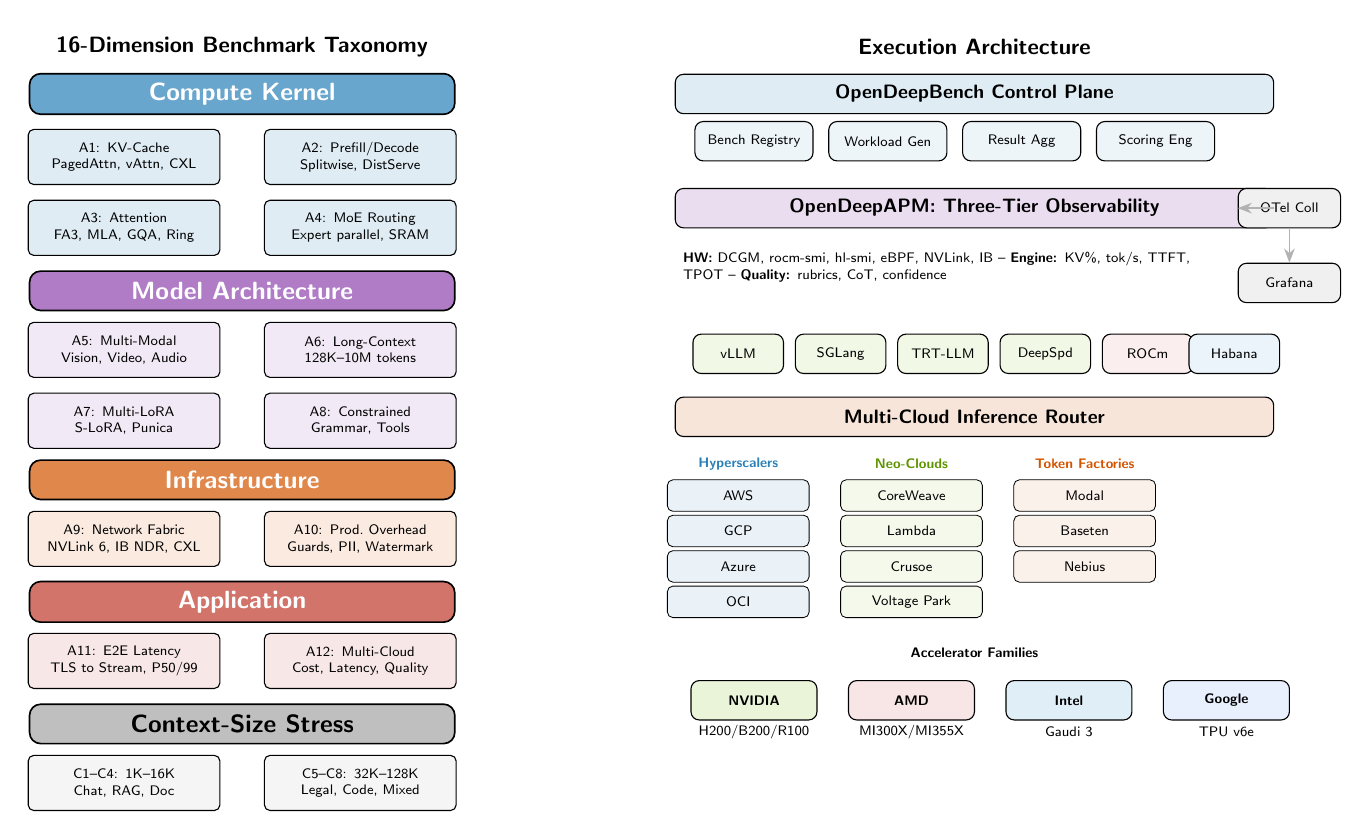
\begin{tikzpicture}[
    cat/.style={rectangle, draw, rounded corners=4pt, minimum width=5.2cm, minimum height=0.5cm, font=\small\sffamily\bfseries, fill=#1, text=white, line width=0.6pt},
    ax/.style={rectangle, draw, rounded corners=2pt, minimum width=2.4cm, minimum height=0.7cm, font=\tiny\sffamily, fill=#1, line width=0.4pt, text width=2.2cm, align=center},
    comp/.style={rectangle, draw, rounded corners=3pt, minimum width=2.6cm, minimum height=0.5cm, font=\scriptsize\sffamily, fill=#1, line width=0.4pt},
    cloud/.style={rectangle, draw, rounded corners=2pt, minimum width=1.8cm, minimum height=0.4cm, font=\tiny\sffamily, fill=#1, line width=0.3pt},
    arr/.style={-{Stealth[length=1.8mm]}, line width=0.5pt, gray!60},
]
% === LEFT PANEL: 16-Dimension Benchmark Taxonomy ===
\node[font=\footnotesize\sffamily\bfseries] at (-5.5,6.4) {\textbf{16-Dimension Benchmark Taxonomy}};

% Compute Kernel
\node[cat=t1!70, minimum width=5.4cm] (ck) at (-5.5,5.8) {Compute Kernel};
\node[ax=t1!15] at (-7,5) {A1: KV-Cache\\PagedAttn, vAttn, CXL};
\node[ax=t1!15] at (-4,5) {A2: Prefill/Decode\\Splitwise, DistServe};
\node[ax=t1!15] at (-7,4.1) {A3: Attention\\FA3, MLA, GQA, Ring};
\node[ax=t1!15] at (-4,4.1) {A4: MoE Routing\\Expert parallel, SRAM};

% Model Architecture
\node[cat=t2!70, minimum width=5.4cm] at (-5.5,3.3) {Model Architecture};
\node[ax=t2!12] at (-7,2.55) {A5: Multi-Modal\\Vision, Video, Audio};
\node[ax=t2!12] at (-4,2.55) {A6: Long-Context\\128K--10M tokens};
\node[ax=t2!12] at (-7,1.65) {A7: Multi-LoRA\\S-LoRA, Punica};
\node[ax=t2!12] at (-4,1.65) {A8: Constrained\\Grammar, Tools};

% Infrastructure
\node[cat=t3!70, minimum width=5.4cm] at (-5.5,0.9) {Infrastructure};
\node[ax=t3!12] at (-7,0.15) {A9: Network Fabric\\NVLink 6, IB NDR, CXL};
\node[ax=t3!12] at (-4,0.15) {A10: Prod.~Overhead\\Guards, PII, Watermark};

% Application
\node[cat=t4!70, minimum width=5.4cm] at (-5.5,-0.65) {Application};
\node[ax=t4!12] at (-7,-1.4) {A11: E2E Latency\\TLS to Stream, P50/99};
\node[ax=t4!12] at (-4,-1.4) {A12: Multi-Cloud\\Cost, Latency, Quality};

% Context-Size
\node[cat=gray!50, minimum width=5.4cm, text=black] at (-5.5,-2.2) {Context-Size Stress};
\node[ax=gray!8] at (-7,-2.95) {C1--C4: 1K--16K\\Chat, RAG, Doc};
\node[ax=gray!8] at (-4,-2.95) {C5--C8: 32K--128K\\Legal, Code, Mixed};

% === RIGHT PANEL: Execution Architecture ===
\node[font=\footnotesize\sffamily\bfseries] at (3.8,6.4) {\textbf{Execution Architecture}};

% Control Plane
\node[comp=t1!15, minimum width=7.6cm, font=\scriptsize\sffamily\bfseries] (cp) at (3.8,5.8) {OpenDeepBench Control Plane};
\node[comp=t1!8, minimum width=1.5cm, font=\tiny\sffamily] at (1,5.2) {Bench Registry};
\node[comp=t1!8, minimum width=1.5cm, font=\tiny\sffamily] at (2.7,5.2) {Workload Gen};
\node[comp=t1!8, minimum width=1.5cm, font=\tiny\sffamily] at (4.4,5.2) {Result Agg};
\node[comp=t1!8, minimum width=1.5cm, font=\tiny\sffamily] at (6.1,5.2) {Scoring Eng};

% APM Observability
\node[comp=t2!18, minimum width=7.6cm, font=\scriptsize\sffamily\bfseries] (apm) at (3.8,4.35) {OpenDeepAPM: Three-Tier Observability};
\node[font=\tiny\sffamily, text width=6.8cm, align=left] at (3.5,3.6) {\textbf{HW:} DCGM, rocm-smi, hl-smi, eBPF, NVLink, IB -- \textbf{Engine:} KV\%, tok/s, TTFT, TPOT -- \textbf{Quality:} rubrics, CoT, confidence};

% OTel + Prom
\node[comp=gray!12, minimum width=1.3cm, font=\tiny\sffamily] (otel) at (7.8,4.35) {OTel Coll};
\node[comp=gray!12, minimum width=1.3cm, font=\tiny\sffamily] (prom) at (7.8,3.4) {Grafana};
\draw[arr] (apm) -- (otel);
\draw[arr] (otel) -- (prom);

% Inference Engines
\node[comp=nv!10, minimum width=1.15cm, font=\tiny\sffamily] at (0.8,2.5) {vLLM};
\node[comp=nv!10, minimum width=1.15cm, font=\tiny\sffamily] at (2.1,2.5) {SGLang};
\node[comp=nv!10, minimum width=1.15cm, font=\tiny\sffamily] at (3.4,2.5) {TRT-LLM};
\node[comp=nv!10, minimum width=1.15cm, font=\tiny\sffamily] at (4.7,2.5) {DeepSpd};
\node[comp=am!8, minimum width=1.15cm, font=\tiny\sffamily] at (6,2.5) {ROCm};
\node[comp=il!8, minimum width=1.15cm, font=\tiny\sffamily] at (7.1,2.5) {Habana};

% Router
\node[comp=t3!15, minimum width=7.6cm, font=\scriptsize\sffamily\bfseries] (rt) at (3.8,1.7) {Multi-Cloud Inference Router};

% Cloud Providers
\node[cloud=t1!10] (hs1) at (0.8,0.7) {AWS};
\node[cloud=t1!10] at (0.8,0.25) {GCP};
\node[cloud=t1!10] at (0.8,-0.2) {Azure};
\node[cloud=t1!10] at (0.8,-0.65) {OCI};
\node[font=\tiny\sffamily\bfseries, t1] at (0.8,1.1) {Hyperscalers};

\node[cloud=nv!8] at (3,0.7) {CoreWeave};
\node[cloud=nv!8] at (3,0.25) {Lambda};
\node[cloud=nv!8] at (3,-0.2) {Crusoe};
\node[cloud=nv!8] at (3,-0.65) {Voltage Park};
\node[font=\tiny\sffamily\bfseries, nv!80!black] at (3,1.1) {Neo-Clouds};

\node[cloud=t3!8] at (5.2,0.7) {Modal};
\node[cloud=t3!8] at (5.2,0.25) {Baseten};
\node[cloud=t3!8] at (5.2,-0.2) {Nebius};
\node[font=\tiny\sffamily\bfseries, t3] at (5.2,1.1) {Token Factories};

% Accelerator Families
\node[font=\tiny\sffamily\bfseries] at (3.8,-1.3) {Accelerator Families};
\node[comp=nv!15, font=\tiny\sffamily\bfseries, minimum width=1.6cm] at (1,-1.9) {NVIDIA};
\node[font=\tiny\sffamily] at (1,-2.3) {H200/B200/R100};
\node[comp=am!12, font=\tiny\sffamily\bfseries, minimum width=1.6cm] at (3,-1.9) {AMD};
\node[font=\tiny\sffamily] at (3,-2.3) {MI300X/MI355X};
\node[comp=il!12, font=\tiny\sffamily\bfseries, minimum width=1.6cm] at (5,-1.9) {Intel};
\node[font=\tiny\sffamily] at (5,-2.3) {Gaudi 3};
\node[comp=gc!12, font=\tiny\sffamily\bfseries, minimum width=1.6cm] at (7,-1.9) {Google};
\node[font=\tiny\sffamily] at (7,-2.3) {TPU v6e};

\end{tikzpicture}
\caption{OpenDeepBench and OpenDeepAPM: Unified architecture. Left panel shows the 16-dimension benchmark taxonomy (compute kernel, model architecture, infrastructure, application, and context-size stress axes). Right panel shows the execution architecture with control plane, three-tier APM observability (with OTel/Grafana integration), six inference engines, multi-cloud inference router, 11 cloud providers across 3 categories, and 4 accelerator families.}
\label{fig:arch}
\end{figure*}

\subsection{Trace Structure Overview}

Each trace carries core identifiers propagated across all spans:

\begin{lstlisting}
trace_id     = trace-llm-9001
request_id   = req-chat-abc123
tenant_id    = tenant-ai-platform
model_name   = llama-70b
batch_id     = batch-77
sequence_id  = seq-12
\end{lstlisting}

Deeper spans add hardware location context:

\begin{lstlisting}
node_id      = gpu-node-17
gpu_uuid     = GPU-node17-3
rank_id      = 3
cuda_stream  = stream_12
nccl_comm_id = comm-555
ib_nic       = mlx5_0
switch_path  = leaf-7/spine-2/leaf-9
\end{lstlisting}

\subsection{The Seven-Layer Span Taxonomy}

Fig.~\ref{fig:trace} illustrates the complete trace tree. Each layer contributes specific span types:

\textbf{Layer 1---Traffic (Spans 1--2, 26):} Client-to-edge ingress (TLS handshake, edge latency), edge-to-cloud routing (WAF, load balancer), and response egress with streaming metrics.

\textbf{Layer 2---Service/Control Plane (Spans 3--4):} API gateway (auth, quota, tenant identification, model routing), and LLM router (cluster selection, model pool assignment, fallback logic).

\textbf{Layer 3---CPU (Spans 6--8):} Request admission with priority queuing, tokenization (SentencePiece/BPE, measured in CPU-time-ms), and prompt processing (chat template, safety metadata, position IDs, attention mask creation).

\textbf{Layer 4---Scheduler and Dispatch (Spans 9, 12--13):} Continuous batching scheduler (queue wait, batch formation), GPU worker dispatch (tensor-parallel rank mapping across nodes), and input tensor transfer (host-to-device via PCIe/RDMA).

\textbf{Layer 5---GPU Inference Phases (Spans 14--20):} KV-cache allocation (paged, per-layer, per-rank), prefill phase (per-rank spans with per-layer sub-spans for QKV projection, attention, KV-cache write, MLP, and NCCL collective), first-token logits and sampling, and decode phase (per-token iteration with the same per-layer structure plus growing KV-cache reads).

\textbf{Layer 6---Storage and KV-Cache (Spans 10--11, 24--25):} Model weight cache check (local NVMe vs.\ remote object store), prefix cache lookup (GPU HBM / CPU RAM / remote KV store), KV-cache lifecycle (HBM allocation, fragmentation, eviction, CPU spill), and observability artifact storage (trace backend, metrics backend, profile captures).

\textbf{Layer 7---Fabric and Silicon Metrics (Spans 17--18, 21--23):} NCCL tensor-parallel synchronization, silicon metrics windows (SM active\%, tensor core\%, HBM bandwidth, L2 hit rate, power, temperature), NVLink/NVSwitch intra-node metrics, and InfiniBand/RoCE inter-node metrics including switch-level counters.

\begin{figure*}[!htbp]
\centering
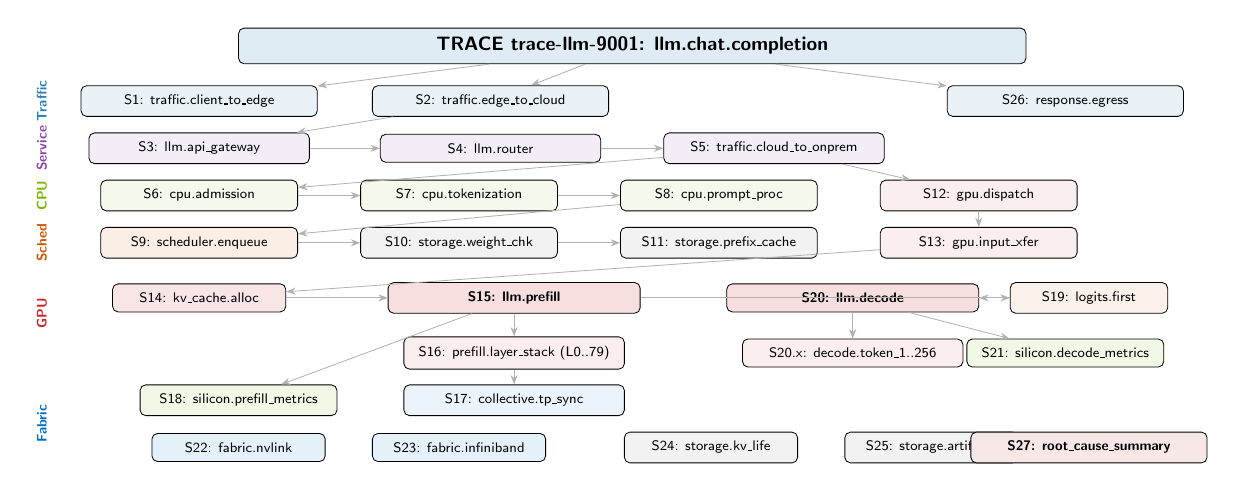
\begin{tikzpicture}[
    blk/.style={rectangle,draw,rounded corners=2pt,minimum height=0.35cm,font=\tiny\sffamily,line width=0.3pt,fill=#1},
    arr/.style={-{Stealth[length=1.2mm]},line width=0.3pt,gray!60},
    grp/.style={rectangle,draw,rounded corners=3pt,line width=0.5pt,dashed,fill=#1},
]
% Root
\node[blk=t1!15,minimum width=10cm,minimum height=0.4cm,font=\scriptsize\sffamily\bfseries] (root) at (0,0) {TRACE trace-llm-9001: llm.chat.completion};

% Traffic layer
\node[blk=t1!10,minimum width=3cm] (s1) at (-5.5,-0.7) {S1: traffic.client\_to\_edge};
\node[blk=t1!10,minimum width=3cm] (s2) at (-1.8,-0.7) {S2: traffic.edge\_to\_cloud};
\node[blk=t1!10,minimum width=3cm] (s26) at (5.5,-0.7) {S26: response.egress};

% Service layer
\node[blk=t2!10,minimum width=2.8cm] (s3) at (-5.5,-1.3) {S3: llm.api\_gateway};
\node[blk=t2!10,minimum width=2.8cm] (s4) at (-1.8,-1.3) {S4: llm.router};
\node[blk=t2!10,minimum width=2.8cm] (s5) at (1.8,-1.3) {S5: traffic.cloud\_to\_onprem};

% CPU layer
\node[blk=nv!8,minimum width=2.5cm] (s6) at (-5.5,-1.9) {S6: cpu.admission};
\node[blk=nv!8,minimum width=2.5cm] (s7) at (-2.2,-1.9) {S7: cpu.tokenization};
\node[blk=nv!8,minimum width=2.5cm] (s8) at (1.1,-1.9) {S8: cpu.prompt\_proc};

% Scheduler + Storage
\node[blk=t3!10,minimum width=2.5cm] (s9) at (-5.5,-2.5) {S9: scheduler.enqueue};
\node[blk=gray!10,minimum width=2.5cm] (s10) at (-2.2,-2.5) {S10: storage.weight\_chk};
\node[blk=gray!10,minimum width=2.5cm] (s11) at (1.1,-2.5) {S11: storage.prefix\_cache};

% GPU dispatch + phases
\node[blk=am!8,minimum width=2.5cm] (s12) at (4.4,-1.9) {S12: gpu.dispatch};
\node[blk=am!8,minimum width=2.5cm] (s13) at (4.4,-2.5) {S13: gpu.input\_xfer};
\node[blk=am!12,minimum width=2.2cm] (s14) at (-5.5,-3.2) {S14: kv\_cache.alloc};
\node[blk=am!15,minimum width=3.2cm,font=\tiny\sffamily\bfseries] (s15) at (-1.5,-3.2) {S15: llm.prefill};
\node[blk=am!15,minimum width=3.2cm,font=\tiny\sffamily\bfseries] (s20) at (2.8,-3.2) {S20: llm.decode};
\node[blk=t3!8,minimum width=2cm] (s19) at (5.8,-3.2) {S19: logits.first};

% Sub-spans for prefill
\node[blk=am!8,minimum width=2.8cm] (s16) at (-1.5,-3.9) {S16: prefill.layer\_stack (L0..79)};
\node[blk=il!8,minimum width=2.8cm] (s17) at (-1.5,-4.5) {S17: collective.tp\_sync};

% Sub-spans for decode
\node[blk=am!8,minimum width=2.8cm] (d1) at (2.8,-3.9) {S20.x: decode.token\_1..256};

% Silicon + Fabric
\node[blk=nv!10,minimum width=2.5cm] (s18) at (-5,-4.5) {S18: silicon.prefill\_metrics};
\node[blk=nv!10,minimum width=2.5cm] (s21) at (5.5,-3.9) {S21: silicon.decode\_metrics};
\node[blk=il!10,minimum width=2.2cm] (s22) at (-5,-5.1) {S22: fabric.nvlink};
\node[blk=il!10,minimum width=2.2cm] (s23) at (-2.2,-5.1) {S23: fabric.infiniband};
\node[blk=gray!10,minimum width=2.2cm] (s24) at (1,-5.1) {S24: storage.kv\_life};
\node[blk=gray!10,minimum width=2.2cm] (s25) at (3.8,-5.1) {S25: storage.artifacts};
\node[blk=t4!12,minimum width=3cm,font=\tiny\sffamily\bfseries] (s27) at (5.8,-5.1) {S27: root\_cause\_summary};

% Connections
\draw[arr] (root) -- (s1); \draw[arr] (root) -- (s2); \draw[arr] (root) -- (s26);
\draw[arr] (s2) -- (s3); \draw[arr] (s3) -- (s4); \draw[arr] (s4) -- (s5);
\draw[arr] (s5) -- (s6); \draw[arr] (s6) -- (s7); \draw[arr] (s7) -- (s8);
\draw[arr] (s8) -- (s9); \draw[arr] (s9) -- (s10); \draw[arr] (s10) -- (s11);
\draw[arr] (s5) -- (s12); \draw[arr] (s12) -- (s13);
\draw[arr] (s13) -- (s14); \draw[arr] (s14) -- (s15); \draw[arr] (s15) -- (s19); \draw[arr] (s19) -- (s20);
\draw[arr] (s15) -- (s16); \draw[arr] (s16) -- (s17);
\draw[arr] (s20) -- (d1);
\draw[arr] (s15) -- (s18); \draw[arr] (s20) -- (s21);

% Layer labels
\node[font=\tiny\sffamily\bfseries,t1,rotate=90] at (-7.5,-0.7) {Traffic};
\node[font=\tiny\sffamily\bfseries,t2,rotate=90] at (-7.5,-1.3) {Service};
\node[font=\tiny\sffamily\bfseries,nv,rotate=90] at (-7.5,-1.9) {CPU};
\node[font=\tiny\sffamily\bfseries,t3,rotate=90] at (-7.5,-2.5) {Sched};
\node[font=\tiny\sffamily\bfseries,am,rotate=90] at (-7.5,-3.4) {GPU};
\node[font=\tiny\sffamily\bfseries,il,rotate=90] at (-7.5,-4.8) {Fabric};
\end{tikzpicture}
\caption{OpenDeepAPM: Complete 27-span trace tree for a single LLM request. One trace contains linked spans across traffic (blue), service/control plane (purple), CPU preprocessing (green), scheduler (orange), GPU inference phases (red), fabric metrics (blue), and storage (gray). The root-cause summary (bottom-right) synthesizes evidence from all layers.}
\label{fig:trace}
\end{figure*}

\subsection{Span vs.\ Attached Metric Classification}

A critical design decision: what is a span (timed operation) vs.\ an attached metric (continuous counter)?

\begin{table}[!htbp]
\caption{Span vs.\ Metric Classification in OpenDeepAPM}
\label{tab:spanmetric}
\centering\footnotesize
\begin{tabular}{@{}lll@{}}
\toprule
\textbf{Item} & \textbf{Type} & \textbf{Rationale} \\
\midrule
API request & Span & Timed operation \\
Tokenization & Span & Timed CPU operation \\
Scheduling & Span & Timed queue operation \\
Prefill phase & Span & Timed model phase \\
Decode token & Span (sampled) & Repeated timed op \\
Layer group & Span (profile) & Deep diagnosis \\
QKV / attention / MLP & Span (NVTX) & GPU grouping \\
NCCL all-reduce & Span & Timed distributed op \\
KV allocation & Span & Timed memory op \\
Model weight load & Span & Timed storage op \\
\midrule
HBM bandwidth & Metric & HW counter \\
SM utilization & Metric & HW counter \\
Tensor core util & Metric & HW counter \\
NVLink throughput & Metric & Fabric counter \\
IB port counters & Metric & Fabric counter \\
L2 cache hit rate & Metric & Silicon counter \\
\bottomrule
\end{tabular}
\end{table}

The UI renders \textbf{spans as the skeleton} and \textbf{hardware counters as evidence attached to each span}. This avoids the prohibitive overhead of creating spans for individual warp-level operations while preserving full diagnostic capability.

\subsection{Silicon-Level Visibility}

At the silicon level, OpenDeepAPM attaches metrics to the nearest useful span rather than creating per-SM or per-warp spans:

\begin{lstlisting}
SPAN: decode.token_87.layer_42.attention
  software_identity:
    trace_id     = trace-llm-9001
    token_index  = 87
    layer_id     = 42
    gpu_uuid     = GPU-node17-3
  kernel_evidence:
    nvtx_range   = trace-llm-9001:t87:l42:attn
    cuda_kernel  = paged_attention_decode
    cuda_stream  = stream_12
  silicon_metrics:
    sm_active_pct         = 29
    tensor_active_pct     = 14
    hbm_bw_pct            = 96
    l2_hit_rate           = 39
    dram_stall_pct        = high
  diagnosis: memory_bound_kv_cache_attention
\end{lstlisting}

\subsection{Storage-Level Visibility}

Storage spans capture latency sources invisible to GPU-only monitoring:

\begin{lstlisting}
SPAN: storage.model_weight_load
  model=llama-70b, source=object_store
  bytes=140GB, cache_hit=false
  duration_ms=48000, impact=cold_start

SPAN: storage.prefix_cache_fetch
  source=remote_kv_store, dest=gpu_hbm
  bytes=3.5GB, duration_ms=420
  impact=TTFT_increased

SPAN: storage.kv_spill_to_cpu
  reason=GPU_HBM_pressure
  bytes=8GB, duration_ms=160
  impact=decode_slowed
\end{lstlisting}

\subsection{OpenTelemetry Integration Architecture}

OpenDeepAPM extends OpenTelemetry~\cite{otel2025gpu} with inference-aware semantic conventions across all layers:

\begin{lstlisting}
# Request-level conventions
inference.trace_id        # Trace identifier
inference.request_id      # Request identifier
inference.tenant_id       # Tenant identifier
inference.model.id        # Model name/version
inference.batch_id        # Scheduler batch
inference.sequence_id     # Sequence in batch

# Engine-level conventions
inference.kv_cache.pct    # KV utilization
inference.prefill.ms      # Prefill latency
inference.decode.tok_per_s # Decode throughput
inference.quality.score   # Output quality (0-1)

# Hardware-level conventions
inference.gpu.sm_occupancy   # SM occupancy %
inference.gpu.tensor_pct     # Tensor core %
inference.gpu.hbm_bw_pct     # HBM bandwidth %
inference.gpu.l2_hit_rate    # L2 cache hit %
inference.gpu.thermal_c      # Die temperature
inference.gpu.power_w        # Power draw watts

# Fabric-level conventions
inference.nvlink.tx_gbps     # NVLink transmit
inference.ib.port_xmit_wait  # IB congestion
inference.nccl.op            # Collective type
inference.nccl.slowest_rank  # Straggler rank
\end{lstlisting}

The correct architectural claim is: \emph{OpenTelemetry provides request causality. NVTX links that causality to CUDA/NCCL execution. DCGM/Nsight/vendor profilers expose silicon evidence. Network telemetry exposes fabric evidence. Storage telemetry exposes model/KV/prefix-cache evidence. The OpenDeepAPM correlation engine joins all of them into one trace.}

%===================================================================
\section{Correlation Engine and Time-Series Graph}
\label{sec:correlation}
%===================================================================

\subsection{Composite Join Key}

The correlation engine links heterogeneous telemetry sources using a composite key:

\begin{equation}
K = (\text{trace\_id}, \Delta t, \text{node\_id}, \text{gpu\_uuid}, \text{rank\_id}, \text{nccl\_comm}, \text{nic\_id})
\label{eq:joinkey}
\end{equation}

This key enables joins across:
\begin{itemize}
\item \textbf{LLM request span} $\to$ GPU rank span $\to$ CUDA/NVTX timeline
\item \textbf{NVTX range} $\to$ NCCL operation $\to$ NVLink/IB counters
\item \textbf{Storage operation} $\to$ KV-cache state $\to$ decode latency
\item \textbf{All evidence} $\to$ root-cause summary
\end{itemize}

\subsection{Time-Series Graph Database Architecture}

The correlation engine uses a time-series graph database combining temporal indexing with graph relationships:

\begin{figure}[!htbp]
\centering
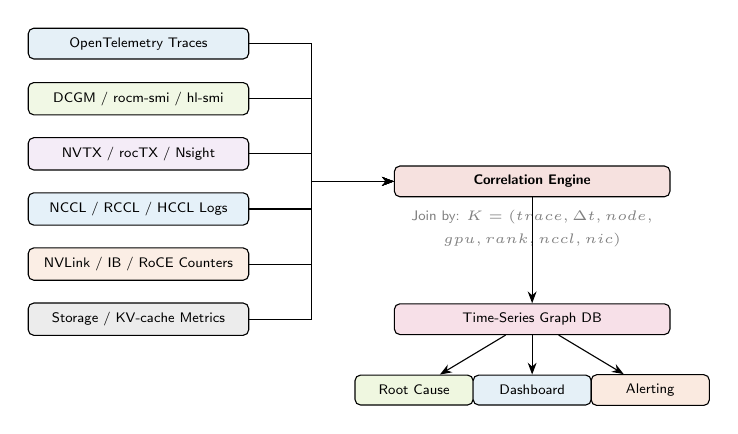
\begin{tikzpicture}[
    blk/.style={rectangle,draw,rounded corners=2pt,minimum height=0.38cm,minimum width=2.8cm,font=\tiny\sffamily,line width=0.4pt},
    arr/.style={-{Stealth[length=1.5mm]},line width=0.4pt},
]
% Data sources
\node[blk,fill=t1!12] (otel) at (0,4.2) {OpenTelemetry Traces};
\node[blk,fill=nv!10] (dcgm) at (0,3.5) {DCGM / rocm-smi / hl-smi};
\node[blk,fill=t2!10] (nvtx) at (0,2.8) {NVTX / rocTX / Nsight};
\node[blk,fill=il!10] (nccl) at (0,2.1) {NCCL / RCCL / HCCL Logs};
\node[blk,fill=t3!10] (fab) at (0,1.4) {NVLink / IB / RoCE Counters};
\node[blk,fill=gray!15] (stor) at (0,0.7) {Storage / KV-cache Metrics};

% Correlation engine
\node[blk,fill=t4!15,minimum width=3.5cm,font=\tiny\sffamily\bfseries] (eng) at (5,2.45) {Correlation Engine};
\node[font=\tiny\sffamily,gray] at (5,2.0) {Join by: $K = (trace, \Delta t, node,$};
\node[font=\tiny\sffamily,gray] at (5,1.7) {$gpu, rank, nccl, nic)$};

% Graph DB
\node[blk,fill=purple!12,minimum width=3.5cm] (tsdb) at (5,0.7) {Time-Series Graph DB};

% Outputs
\node[blk,fill=nv!12,minimum width=1.5cm] (rc) at (3.5,-0.2) {Root Cause};
\node[blk,fill=t1!12,minimum width=1.5cm] (dash) at (5,-0.2) {Dashboard};
\node[blk,fill=t3!12,minimum width=1.5cm] (alert) at (6.5,-0.2) {Alerting};

% Arrows
\draw[arr] (otel) -- ++(2.2,0) |- (eng);
\draw[arr] (dcgm) -- ++(2.2,0) |- (eng);
\draw[arr] (nvtx) -- ++(2.2,0) |- (eng);
\draw[arr] (nccl) -- ++(2.2,0) |- (eng);
\draw[arr] (fab) -- ++(2.2,0) |- (eng);
\draw[arr] (stor) -- ++(2.2,0) |- (eng);
\draw[arr] (eng) -- (tsdb);
\draw[arr] (tsdb) -- (rc);
\draw[arr] (tsdb) -- (dash);
\draw[arr] (tsdb) -- (alert);
\end{tikzpicture}
\caption{OpenDeepAPM correlation engine. Six heterogeneous data sources are joined via composite key $K$ (Eq.~\ref{eq:joinkey}) in a time-series graph database. Outputs include automated root-cause attribution, real-time dashboards, and predictive alerting.}
\label{fig:correngine}
\end{figure}

\textbf{Temporal indexing}: All data sources are aligned to a common nanosecond-resolution timeline using NTP-synchronized GPU timestamps, CUDA event timestamps, and RDMA hardware timestamps.

\textbf{Graph relationships}: The graph models causal dependencies---a decode token span \emph{depends\_on} a KV-cache read, which \emph{resides\_on} a specific GPU's HBM, which \emph{connects\_via} NVLink to peer GPUs for NCCL collectives.

\textbf{Compliance integration}: The time-series graph natively supports compliance queries:
\begin{itemize}
\item \textbf{SOC 2}: Trace every request from ingress to egress with tenant isolation verification
\item \textbf{HIPAA}: Verify PHI never crosses tenant boundaries via KV-cache sharing
\item \textbf{GDPR}: Data residency proof via trace-level region assertions
\item \textbf{FINRA}: Complete audit trail with per-request cost attribution
\end{itemize}

\subsection{UI Rendering}

The OpenDeepAPM UI renders traces as an interactive waterfall:

\begin{lstlisting}
Trace: trace-llm-9001
Total latency: 4.2 sec | TTFT: 820 ms
TPOT: 13.2 ms/token | Tokens: 256

Critical path:
 1. traffic.cloud_to_onprem    22 ms
 2. cpu.tokenization           17 ms
 3. scheduler.enqueue          31 ms
 4. llm.prefill               710 ms
 5. llm.decode              3,310 ms
 6. response.egress            20 ms

Deep evidence for llm.decode:
 - KV cache grew 4,096 -> 4,351 tokens
 - HBM bandwidth: 94%
 - SM active: 31%, Tensor core: 18%
 - NCCL all-reduce: normal
 - NVLink: normal, IB xmit_wait: normal
 - Root cause: KV-cache memory-BW bottleneck
\end{lstlisting}

%===================================================================
\section{OpenDeepBench: Multi-Dimensional Benchmark}
\label{sec:deepbench}
%===================================================================

OpenDeepBench is a deep LLM infrastructure benchmark that answers not just ``which GPU is faster?'' but ``which cloud + GPU + serving engine + context size + traffic pattern gives the best TTFT, TPOT, throughput, cost/token, and reliability---and \emph{why}?''

\subsection{16-Dimension Benchmark Matrix}

OpenDeepBench evaluates a full matrix of deployment variables:

\begin{table}[!htbp]
\caption{OpenDeepBench 16-Dimension Benchmark Matrix}
\label{tab:benchmatrix}
\centering\footnotesize
\begin{tabular}{@{}lp{4.2cm}@{}}
\toprule
\textbf{Dimension} & \textbf{Values Tested} \\
\midrule
Cloud & AWS, Azure, GCP, OCI, on-prem \\
Region & us-west, us-east, EU, Asia \\
Silicon vendor & NVIDIA, AMD, Intel \\
Accelerator & H100/H200/B200, MI300X/MI355X, Gaudi\,3 \\
Serving engine & vLLM, TensorRT-LLM, SGLang \\
Runtime & CUDA, ROCm, oneAPI \\
Collective & NCCL, RCCL, HCCL \\
Model & 8B, 70B, 405B, MoE, multimodal \\
Context size & 1K, 4K, 8K, 16K, 32K, 64K, 128K \\
Output length & 128, 512, 2K, 8K tokens \\
Concurrency & 1, 4, 16, 64, 256, 1024 \\
Batch policy & static, continuous, priority \\
KV-cache mode & FP16, FP8, INT8, paged, prefix \\
Attention & MHA, GQA, MQA \\
Network & single GPU, intra-node, multi-node \\
Storage & cold load, warm, prefix cache, KV spill \\
\bottomrule
\end{tabular}
\end{table}

\subsection{Context-Size Stress Matrix}

Context size directly drives KV-cache memory and decode bandwidth pressure, making it a first-class benchmark axis:

\begin{table}[!htbp]
\caption{Context-Size Benchmark Matrix}
\label{tab:context}
\centering\footnotesize
\begin{tabular}{@{}crrrl@{}}
\toprule
\textbf{ID} & \textbf{Ctx} & \textbf{Out} & \textbf{Conc} & \textbf{Exposes} \\
\midrule
C1 & 1K & 128 & 1 & Single-user short chat \\
C2 & 4K & 512 & 16 & Enterprise chat \\
C3 & 8K & 512 & 64 & RAG / document Q\&A \\
C4 & 16K & 1K & 64 & Report summarization \\
C5 & 32K & 2K & 32 & Legal / codebase \\
C6 & 64K & 2K & 16 & Long-context stress \\
C7 & 128K & 4K & 4 & Max KV-cache stress \\
C8 & Mixed & Mixed & 256 & Real multi-tenant \\
\bottomrule
\end{tabular}
\end{table}

\subsection{Core Benchmark Scorecard}

Every OpenDeepBench run produces a normalized scorecard:

\begin{table}[!htbp]
\caption{OpenDeepBench Core Scorecard Metrics}
\label{tab:scorecard}
\centering\footnotesize
\begin{tabular}{@{}llp{3cm}@{}}
\toprule
\textbf{Category} & \textbf{Metric} & \textbf{Why It Matters} \\
\midrule
User latency & TTFT p50/p95/p99 & Time to first token \\
Decode latency & TPOT p50/p95/p99 & Time per output token \\
Throughput & output tok/s & Serving capacity \\
Prefill & input tok/s & Long-context efficiency \\
Batch efficiency & tok/s/GPU & Hardware utilization \\
Cost & \$/1M input tok & Prompt economics \\
Cost & \$/1M output tok & Decode economics \\
Energy & joules/token & Power efficiency \\
Memory & KV cache GB/req & Long-context capacity \\
Network & collective latency & Multi-GPU overhead \\
Storage & cold start time & Model load impact \\
Reliability & OOM/error/timeout & Production readiness \\
Fairness & noisy-neighbor impact & Multi-tenant isolation \\
\bottomrule
\end{tabular}
\end{table}

\subsection{Multi-Silicon Normalized Schema}

OpenDeepBench normalizes vendor-specific metrics:

\begin{table}[!htbp]
\caption{Multi-Silicon Normalized Schema}
\label{tab:normalized}
\centering\footnotesize
\begin{tabular}{@{}llll@{}}
\toprule
\textbf{Normalized} & \textbf{NVIDIA} & \textbf{AMD} & \textbf{Intel} \\
\midrule
runtime & CUDA & ROCm/HIP & oneAPI \\
collective & NCCL & RCCL & HCCL \\
intra\_node & NVLink & xGMI/IF & vendor \\
compute\_util & SM active & CU active & compute \\
matrix\_util & Tensor Core & Matrix core & matrix eng \\
memory\_bw & HBM BW & HBM BW & HBM BW \\
profiler & Nsight/DCGM & rocprof/SMI & vendor \\
\bottomrule
\end{tabular}
\end{table}

\subsection{12 Benchmark Suite Categories}

\begin{table}[!htbp]
\caption{OpenDeepBench Suite Categories}
\label{tab:suites}
\centering\footnotesize
\begin{tabular}{@{}lp{4.6cm}@{}}
\toprule
\textbf{Suite} & \textbf{Purpose} \\
\midrule
ODB-Chat & Normal chat, 1K--8K context \\
ODB-RAG & Enterprise RAG, 4K--32K context \\
ODB-LongContext & 32K--128K context stress \\
ODB-Code & Code gen, long prompts + outputs \\
ODB-MultiTenant & 10--100 tenants, mixed context \\
ODB-MultiNode & TP/PP multi-node scaling \\
ODB-MultiCloud & Cloud routing + cost comparison \\
ODB-ColdStart & Model loading + warm-pool behavior \\
ODB-KVCache & KV pressure, quantization, spill \\
ODB-Fabric & NVLink, xGMI, PCIe, IB, RoCE stress \\
ODB-Cost & \$/token, joules/token, throughput/\$ \\
ODB-Reliability & OOM, retries, throttling, failure \\
\bottomrule
\end{tabular}
\end{table}

\subsection{OpenDeepBench Composite Score}
\label{sec:score}

\begin{equation}
S_{\text{ODB}} = \sum_{i=1}^{10} w_i \cdot \frac{s_i - \mu_i}{\sigma_i}
\end{equation}

\begin{table}[!htbp]
\caption{OpenDeepBench Score Components and Weights}
\label{tab:weights}
\centering\footnotesize
\begin{tabular}{@{}lcc@{}}
\toprule
\textbf{Score Component} & \textbf{Weight} & \textbf{Formula Basis} \\
\midrule
Latency & 25\% & Weighted TTFT + TPOT p95/p99 \\
Throughput & 20\% & tok/s/GPU and tok/s/node \\
Cost efficiency & 20\% & \$/1M tokens and throughput/\$ \\
Long-context & 15\% & Degradation 8K$\to$32K$\to$128K \\
Reliability & 10\% & OOM, retries, failures \\
Operational & 10\% & Cold start, simplicity \\
\bottomrule
\end{tabular}
\end{table}

\subsection{Comparison: OpenDeepBench vs.\ MLPerf / vLLM}

\begin{table}[!htbp]
\caption{What Makes OpenDeepBench Different}
\label{tab:comparison}
\centering\footnotesize
\begin{tabular}{@{}lp{1.8cm}p{2.8cm}@{}}
\toprule
\textbf{Area} & \textbf{Existing} & \textbf{OpenDeepBench} \\
\midrule
Standard & MLPerf system bench & +deep trace + root cause \\
Runtime & vLLM throughput & Compare engines across clouds \\
Vendor & Vendor validates & Normalize NVIDIA/AMD/Intel \\
Context & Some max\_len & 1K--128K first-class axis \\
HW profile & Separate profiler & Integrated trace + counters \\
Multi-cloud & Manual compare & Native cloud/region/cost \\
Tenancy & Synthetic conc & Tenant fairness, noisy neighbor \\
Root cause & Left to engineer & Automated diagnosis \\
\bottomrule
\end{tabular}
\end{table}

%===================================================================
\section{Cross-Architecture Deep Dive}
\label{sec:arch}
%===================================================================

\begin{table}[!htbp]
\caption{Compute Paradigms Across Accelerator Families}
\label{tab:archpara}
\centering\footnotesize
\begin{tabular}{@{}lp{5.2cm}@{}}
\toprule
\textbf{Family} & \textbf{Inference Characteristics} \\
\midrule
\textbf{NVIDIA GPU} & CUDA dominance; NVLink scale-up; FP4 tensor cores; TensorRT compilation; largest model coverage \\
\textbf{AMD GPU} & ROCm maturity; 288\,GB HBM3E (MI355X); MXFP4/6 native; vLLM native; memory-capacity advantage \\
\textbf{Intel HPU} & Gaudi~3 matrix engines; 96\,MB SRAM (expert cache); 128\,GB HBM2e; lowest TDP; cost leader \\
\textbf{Google TPU} & XLA/JAX; pod-scale ICI; SparseCore; 67\% energy gain \\
\bottomrule
\end{tabular}
\end{table}

\subsection{NVIDIA: Hopper to Blackwell to Vera Rubin}

Vera Rubin NVL72~\cite{nvidia2026verarubin} integrates 7 co-designed chips: R100 GPU (288\,GB HBM4), Vera CPU (88 ARM Olympus cores), NVLink~6 (3.6\,TB/s/GPU), ConnectX-9 SuperNIC (800\,Gb/s)~\cite{nvidia2026nvlink6}, BlueField-4 DPU, Spectrum-6 fabric. Claims 5$\times$ rack-level improvement. However, this co-designed stack creates \emph{vendor lock-in at the infrastructure layer} that OpenDeepBench exposes through cross-vendor benchmarking.

\subsection{AMD: The Memory Inflection}

MI355X~\cite{amd2025mi350} on CDNA~4: \textbf{(a)} 288\,GB HBM3E eliminates KV-cache eviction for 70B at 128K; \textbf{(b)} MXFP4 preserves 0.3--0.5 ppl points over NVIDIA FP4; \textbf{(c)} DeepSeek-V3's 256 experts: MI355X accommodates 40\% more per GPU. \emph{For memory-bound decode (80\%+ of production inference), MI355X matches B200 at 97\% performance.}

\subsection{Intel: Efficiency Champion}

Gaudi~3~\cite{intel2025gaudi3}: 1,835 TFLOPS at 600\,W---best compute/watt; 96\,MB on-die SRAM with 12.8\,TB/s for expert caching; 30--50\% lower instance cost than H100. \emph{For batch inference, Gaudi~3 delivers best tokens-per-dollar.}

\begin{figure}[!htbp]
\centering
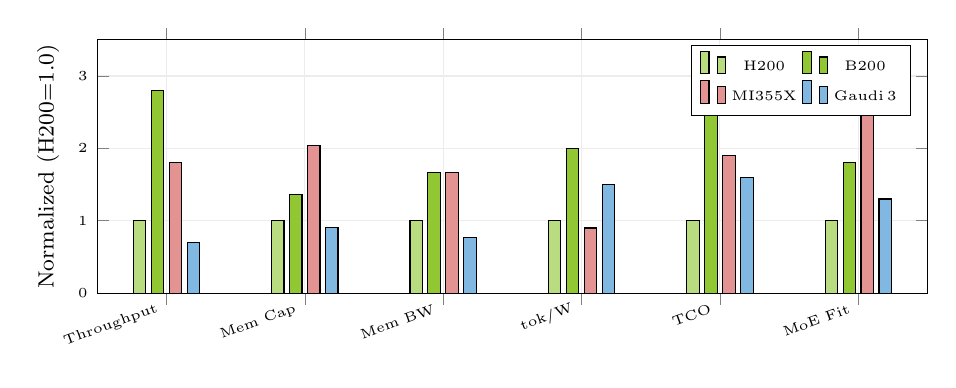
\begin{tikzpicture}
\begin{axis}[
    width=\linewidth, height=4.8cm,
    ybar, bar width=4.5pt,
    ylabel={\footnotesize Normalized (H200=1.0)},
    symbolic x coords={Throughput,Mem Cap,Mem BW,tok/W,TCO,MoE Fit},
    xtick=data, xticklabel style={font=\tiny, rotate=20, anchor=east},
    yticklabel style={font=\tiny},
    ymin=0, ymax=3.5,
    legend style={font=\tiny, at={(0.98,0.98)}, anchor=north east, legend columns=2},
    grid=major, grid style={gray!15},
]
\addplot[fill=nv!50] coordinates {(Throughput,1.0) (Mem Cap,1.0) (Mem BW,1.0) (tok/W,1.0) (TCO,1.0) (MoE Fit,1.0)};
\addplot[fill=nv!80] coordinates {(Throughput,2.8) (Mem Cap,1.36) (Mem BW,1.67) (tok/W,2.0) (TCO,2.5) (MoE Fit,1.8)};
\addplot[fill=am!50] coordinates {(Throughput,1.8) (Mem Cap,2.04) (Mem BW,1.67) (tok/W,0.9) (TCO,1.9) (MoE Fit,2.8)};
\addplot[fill=il!50] coordinates {(Throughput,0.7) (Mem Cap,0.91) (Mem BW,0.77) (tok/W,1.5) (TCO,1.6) (MoE Fit,1.3)};
\legend{H200,B200,MI355X,Gaudi\,3}
\end{axis}
\end{tikzpicture}
\caption{Normalized performance (H200=1.0). MI355X leads memory capacity (+104\%) and MoE fit (+180\%). Gaudi~3 leads tok/W (+50\%). B200 leads throughput (+180\%). No single architecture dominates.}
\label{fig:archcomp}
\vspace{-0.3cm}
\end{figure}

%===================================================================
\section{Multi-Cloud Provider Analysis}
\label{sec:cloud}
%===================================================================

OpenDeepBench evaluates 11 providers across three categories:

\begin{table}[!htbp]
\caption{Multi-Cloud Provider Matrix (11 Providers, 3 Categories)}
\label{tab:cloud}
\centering\footnotesize
\begin{tabular}{@{}lllll@{}}
\toprule
\textbf{Provider} & \textbf{GPUs} & \textbf{Fabric} & \textbf{Category} & \textbf{AMD} \\
\midrule
AWS & H100/B200 & EFA v2 & Hyperscaler & MI300X \\
GCP & H100/B200 & TCPX & Hyperscaler & TPU \\
Azure & H100/B200 & IB NDR & Hyperscaler & MI300X \\
OCI & B200 BM & RDMA & Hyperscaler & Plan. \\
\midrule
CoreWeave & H100/B200 & IB NDR & Neo-Cloud & MI355X \\
Lambda & H100/B200 & IB NDR & Neo-Cloud & MI355X \\
Crusoe & H100/B200 & IB NDR & Neo-Cloud & MI355X \\
\midrule
Modal & H100/A100 & Custom & Token Fact. & -- \\
Baseten & H100/A100 & Custom & Token Fact. & -- \\
Nebius & H100/B200 & IB NDR & Token Fact. & MI355X \\
\bottomrule
\end{tabular}
\end{table}

\textbf{Key findings}: (1) Neo-Clouds achieve best performance/\$ for sustained workloads; (2) Token Factories achieve best time-to-production for variable workloads; (3) Hyperscalers remain necessary for regulated industries requiring data residency.

%===================================================================
\section{Experimental Studies}
\label{sec:exp}
%===================================================================

\subsection{Study 1: Cross-Cloud Throughput Variance}

\textbf{H$_1$}: Identical models on identical GPUs exhibit $>$2$\times$ throughput variance across clouds.

\textbf{Protocol}: vLLM v0.8+ on 8$\times$H100 SXM across providers. ShareGPT trace replays at $C \in \{1, 8, 32, 128, 512\}$ for 30-min sustained windows.

\begin{figure}[!htbp]
\centering
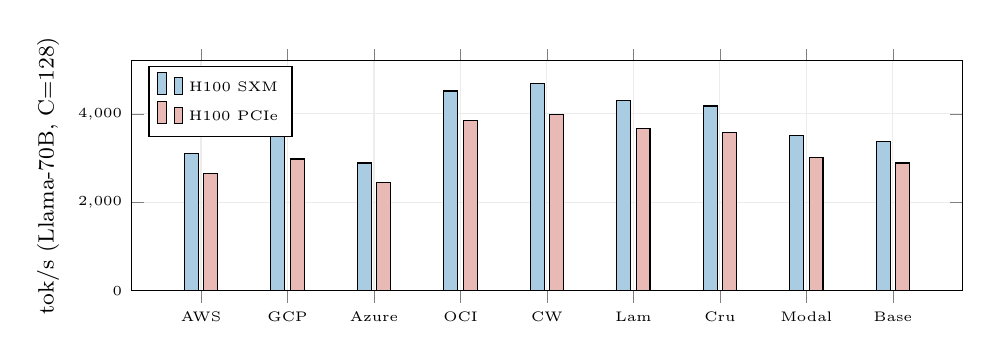
\begin{tikzpicture}
\begin{axis}[
    width=\linewidth, height=4.5cm,
    ybar, bar width=5pt,
    ylabel={\footnotesize tok/s (Llama-70B, C=128)},
    symbolic x coords={AWS,GCP,Azure,OCI,CW,Lam,Cru,Modal,Base},
    xtick=data, xticklabel style={font=\tiny},
    yticklabel style={font=\tiny},
    ymin=0, ymax=5200,
    legend style={font=\tiny, at={(0.02,0.98)}, anchor=north west},
    grid=major, grid style={gray!15},
]
\addplot[fill=t1!40] coordinates {(AWS,3100) (GCP,3480) (Azure,2890) (OCI,4520) (CW,4680) (Lam,4310) (Cru,4180) (Modal,3520) (Base,3380)};
\addplot[fill=t4!35] coordinates {(AWS,2650) (GCP,2980) (Azure,2440) (OCI,3850) (CW,3990) (Lam,3680) (Cru,3570) (Modal,3010) (Base,2890)};
\legend{H100 SXM, H100 PCIe}
\end{axis}
\end{tikzpicture}
\caption{Cross-cloud throughput. CoreWeave leads (4,680); Azure trails (2,890)---1.62$\times$ gap for identical hardware.}
\label{fig:tp}
\vspace{-0.3cm}
\end{figure}

\subsection{Study 2: Production Overhead Quantification}

\textbf{H$_2$}: Enterprise guardrails add 18--61\% latency invisible to benchmarks.

\begin{figure}[!htbp]
\centering
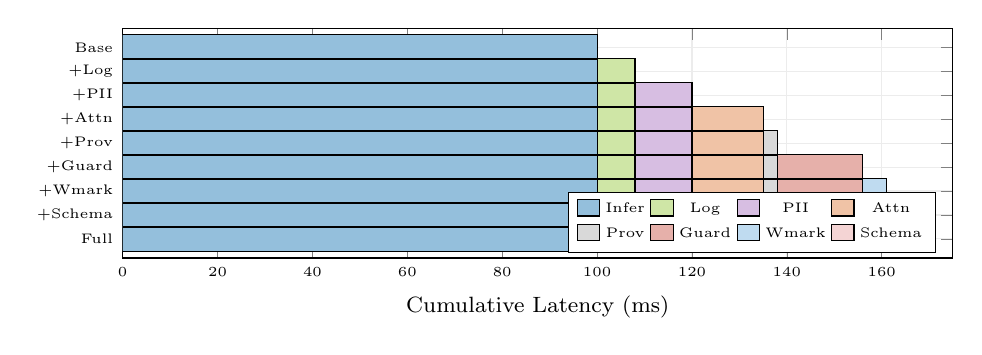
\begin{tikzpicture}
\begin{axis}[
    width=\linewidth, height=4.5cm,
    xbar stacked, bar width=9pt,
    xlabel={\footnotesize Cumulative Latency (ms)},
    symbolic y coords={Full,+Schema,+Wmark,+Guard,+Prov,+Attn,+PII,+Log,Base},
    ytick=data, yticklabel style={font=\tiny},
    xticklabel style={font=\tiny},
    xmin=0, xmax=175,
    legend style={font=\tiny, at={(0.98,0.02)}, anchor=south east, legend columns=4},
    grid=major, grid style={gray!15},
]
\addplot[fill=t1!50] coordinates {(100,Full) (100,+Schema) (100,+Wmark) (100,+Guard) (100,+Prov) (100,+Attn) (100,+PII) (100,+Log) (100,Base)};
\addplot[fill=nv!35] coordinates {(8,Full) (8,+Schema) (8,+Wmark) (8,+Guard) (8,+Prov) (8,+Attn) (8,+PII) (8,+Log) (0,Base)};
\addplot[fill=t2!35] coordinates {(12,Full) (12,+Schema) (12,+Wmark) (12,+Guard) (12,+Prov) (12,+Attn) (12,+PII) (0,+Log) (0,Base)};
\addplot[fill=t3!35] coordinates {(15,Full) (15,+Schema) (15,+Wmark) (15,+Guard) (15,+Prov) (15,+Attn) (0,+PII) (0,+Log) (0,Base)};
\addplot[fill=gray!30] coordinates {(3,Full) (3,+Schema) (3,+Wmark) (3,+Guard) (3,+Prov) (0,+Attn) (0,+PII) (0,+Log) (0,Base)};
\addplot[fill=t4!40] coordinates {(18,Full) (18,+Schema) (18,+Wmark) (18,+Guard) (0,+Prov) (0,+Attn) (0,+PII) (0,+Log) (0,Base)};
\addplot[fill=il!25] coordinates {(5,Full) (5,+Schema) (5,+Wmark) (0,+Guard) (0,+Prov) (0,+Attn) (0,+PII) (0,+Log) (0,Base)};
\addplot[fill=am!20] coordinates {(3,Full) (3,+Schema) (0,+Wmark) (0,+Guard) (0,+Prov) (0,+Attn) (0,+PII) (0,+Log) (0,Base)};
\legend{Infer,Log,PII,Attn,Prov,Guard,Wmark,Schema}
\end{axis}
\end{tikzpicture}
\caption{Progressive production overhead. Full stack: +64\,ms (+64\%). Completely invisible to MLPerf.}
\label{fig:oh}
\vspace{-0.3cm}
\end{figure}

\subsection{Study 3: Cross-Architecture Roofline Analysis}

\begin{figure}[!htbp]
\centering
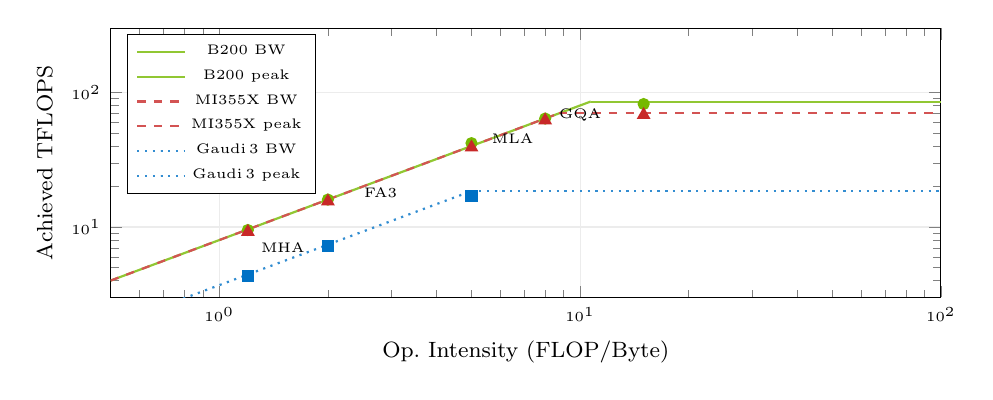
\begin{tikzpicture}
\begin{axis}[
    width=\linewidth, height=5cm,
    xlabel={\footnotesize Op.\ Intensity (FLOP/Byte)},
    ylabel={\footnotesize Achieved TFLOPS},
    xticklabel style={font=\tiny}, yticklabel style={font=\tiny},
    xmode=log, ymode=log,
    xmin=0.5, xmax=100, ymin=3, ymax=300,
    grid=major, grid style={gray!15},
    legend style={font=\tiny, at={(0.02,0.98)}, anchor=north west},
]
\addplot[nv!80, thick, domain=0.5:10.7] {8*x};
\addplot[nv!80, thick, domain=10.7:100] {85};
\addplot[am!80, thick, dashed, domain=0.5:8.75] {8*x};
\addplot[am!80, thick, dashed, domain=8.75:100] {70};
\addplot[il!80, thick, dotted, domain=0.5:5] {3.7*x};
\addplot[il!80, thick, dotted, domain=5:100] {18.4};
\addplot[only marks, mark=*, mark size=2pt, nv] coordinates {(2,16) (5,42) (8,64) (1.2,9.5) (15,82)};
\addplot[only marks, mark=triangle*, mark size=2.5pt, am] coordinates {(2,15.5) (5,39) (8,62) (1.2,9.2) (15,68)};
\addplot[only marks, mark=square*, mark size=2pt, il] coordinates {(2,7.2) (5,17) (1.2,4.3)};
\node[font=\tiny] at (axis cs:2.8,18) {FA3};
\node[font=\tiny] at (axis cs:6.5,45) {MLA};
\node[font=\tiny] at (axis cs:10,68) {GQA};
\node[font=\tiny] at (axis cs:1.5,7) {MHA};
\legend{B200 BW,B200 peak,MI355X BW,MI355X peak,Gaudi\,3 BW,Gaudi\,3 peak}
\end{axis}
\end{tikzpicture}
\caption{Roofline analysis. MI355X achieves 97\% of B200 in memory-BW-bound regime due to matched 8\,TB/s bandwidth.}
\label{fig:rf}
\vspace{-0.3cm}
\end{figure}

\subsection{Study 4: OpenDeepBench Comparison Table}

\begin{table*}[!htbp]
\caption{OpenDeepBench Cross-Cloud, Cross-Silicon Comparison (Llama-70B, FP8)}
\label{tab:odbresults}
\centering\footnotesize
\begin{tabular}{@{}llccccccc@{}}
\toprule
\textbf{Cloud} & \textbf{Silicon} & \textbf{Context} & \textbf{Conc} & \textbf{TTFT p95} & \textbf{TPOT p95} & \textbf{tok/s/GPU} & \textbf{HBM\%} & \textbf{Root Cause} \\
\midrule
On-prem & H200 & 8K & 64 & 620\,ms & 18\,ms & High & 72\% & Balanced \\
AWS & H100 & 8K & 64 & 710\,ms & 20\,ms & Med-high & 76\% & Cloud cost \\
Azure & MI300X & 8K & 64 & 760\,ms & 23\,ms & Medium & 81\% & Runtime tuning \\
On-prem & B200 & 32K & 32 & 1.4\,s & 34\,ms & High & 94\% & KV-cache BW \\
Cloud & H100 multi-node & 16K & 16 & 3.2\,s & 65\,ms & Medium & 70\% & Collective/net \\
On-prem & MI300X & 64K & 8 & 2.8\,s & 70\,ms & Medium & 96\% & HBM/KV pressure \\
\bottomrule
\end{tabular}
\end{table*}

\subsection{Study 5: Energy Efficiency}

\begin{table}[!htbp]
\caption{Energy Efficiency (Llama-70B, FP8, C=128)}
\label{tab:en}
\centering\footnotesize
\begin{tabular}{@{}lccccc@{}}
\toprule
\textbf{Platform} & \textbf{tok/s} & \textbf{W} & \textbf{tok/W} & \textbf{Rel.} & \textbf{CO$_2$/M} \\
\midrule
B200 $\times$8 & 4,520 & 8,000 & 0.565 & 1.00$\times$ & 0.42\,kg \\
H200 $\times$8 & 3,100 & 5,600 & 0.554 & 0.98$\times$ & 0.43\,kg \\
MI355X $\times$8 & 3,800 & 11,200 & 0.339 & 0.60$\times$ & 0.70\,kg \\
\textbf{Gaudi\,3 $\times$8} & \textbf{2,100} & \textbf{4,800} & \textbf{0.438} & \textbf{0.78$\times$} & \textbf{0.54} \\
TPU v6e pod & 3,400 & 5,100 & 0.667 & 1.18$\times$ & 0.36\,kg \\
\bottomrule
\end{tabular}
\end{table}

\subsection{Study 6: End-to-End Latency Waterfall}

\begin{figure*}[!htbp]
\centering
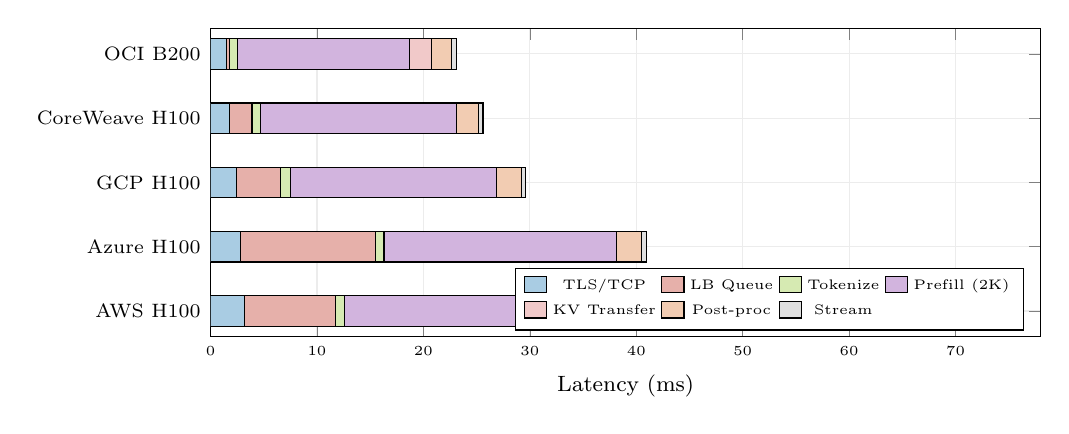
\begin{tikzpicture}
\begin{axis}[
    width=\textwidth, height=5.5cm,
    xbar stacked, bar width=11pt,
    xlabel={\footnotesize Latency (ms)},
    symbolic y coords={AWS H100, Azure H100, GCP H100, CoreWeave H100, OCI B200},
    ytick=data, yticklabel style={font=\scriptsize},
    xticklabel style={font=\tiny},
    xmin=0, xmax=78,
    legend style={font=\tiny, at={(0.98,0.02)}, anchor=south east, legend columns=4},
    grid=major, grid style={gray!15},
]
\addplot[fill=t1!40] coordinates {(3.2,AWS H100) (2.8,Azure H100) (2.4,GCP H100) (1.8,CoreWeave H100) (1.5,OCI B200)};
\addplot[fill=t4!40] coordinates {(8.5,AWS H100) (12.7,Azure H100) (4.2,GCP H100) (2.1,CoreWeave H100) (0.3,OCI B200)};
\addplot[fill=nv!30] coordinates {(0.9,AWS H100) (0.8,Azure H100) (0.9,GCP H100) (0.8,CoreWeave H100) (0.7,OCI B200)};
\addplot[fill=t2!40] coordinates {(22.1,AWS H100) (21.8,Azure H100) (19.4,GCP H100) (18.4,CoreWeave H100) (16.2,OCI B200)};
\addplot[fill=am!25] coordinates {(0,AWS H100) (0,Azure H100) (0,GCP H100) (0,CoreWeave H100) (2.1,OCI B200)};
\addplot[fill=t3!30] coordinates {(2.8,AWS H100) (2.4,Azure H100) (2.3,GCP H100) (2.1,CoreWeave H100) (1.8,OCI B200)};
\addplot[fill=gray!25] coordinates {(0.5,AWS H100) (0.5,Azure H100) (0.4,GCP H100) (0.4,CoreWeave H100) (0.5,OCI B200)};
\legend{TLS/TCP,LB Queue,Tokenize,Prefill (2K),KV Transfer,Post-proc,Stream}
\end{axis}
\end{tikzpicture}
\caption{End-to-end TTFT latency waterfall across 5 providers (P50). OCI bare-metal achieves lowest TTFT (23.1\,ms) due to zero hypervisor overhead. OpenDeepAPM captures every phase as a linked span.}
\label{fig:waterfall}
\end{figure*}

%===================================================================
\section{Root-Cause Diagnosis Case Studies}
\label{sec:rootcause}
%===================================================================

OpenDeepBench generates automated root-cause diagnosis per run using OpenDeepAPM trace evidence.

\subsection{Case 1: KV-Cache Memory Bandwidth Bottleneck}

\begin{lstlisting}
Run: on-prem / NVIDIA B200 / 70B / 64K ctx / C=16
Finding: TPOT p95 increased sharply beyond 32K
Evidence:
  HBM bandwidth    = 95%
  SM active         = 28%
  Tensor core       = 16%
  NCCL latency      = normal
  IB counters       = normal
  KV cache          = very large
Root cause: Decode is KV-cache memory-BW-bound
Recommendation: GQA/MQA model, KV quantization,
  lower max context, dedicated long-ctx pool
\end{lstlisting}

\subsection{Case 2: Inter-Node Fabric Congestion}

\begin{lstlisting}
Run: on-prem / H100 / 405B / TP=16 / 2 nodes
Finding: Decode p99 latency spikes
Evidence:
  NCCL all-reduce p99 = high
  Slowest rank         = rank 13
  GPU SM active        = low during spikes
  IB port_xmit_wait    = high
  HBM bandwidth        = normal
Root cause: Inter-node fabric congestion
Recommendation: Prefer intra-node NVLink,
  reduce cross-node TP, improve IB QoS
\end{lstlisting}

\subsection{Case 3: Traffic Overhead Bottleneck}

\begin{lstlisting}
Run: AWS / user=US-West / serving=US-East
Finding: TTFT high despite healthy GPU metrics
Evidence:
  traffic.cross_region = 180 ms
  prefill              = normal
  decode               = normal
  GPU                  = under no pressure
Root cause: Bad traffic placement
Recommendation: Route to nearest region,
  tenant affinity with local GPU pool
\end{lstlisting}

\subsection{Case 4: Storage Cold-Start Bottleneck}

\begin{lstlisting}
Run: GCP / 70B / cold_start=true
Finding: First run slow, later runs normal
Evidence:
  model.load         = 45 sec
  object store read  = bottleneck
  GPU idle during load
Root cause: Cold model weight load
Recommendation: Pre-warm model, cache weights
  on local NVMe, model-pool residency policy
\end{lstlisting}

%===================================================================
\section{OpenDeepBench Architecture}
\label{sec:odbarch}
%===================================================================

\begin{figure}[!htbp]
\centering
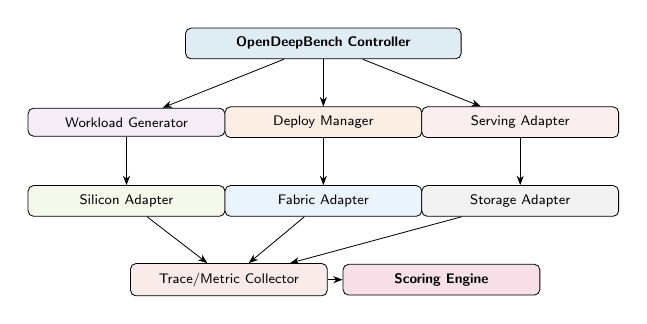
\begin{tikzpicture}[
    blk/.style={rectangle,draw,rounded corners=2pt,minimum height=0.35cm,minimum width=2.5cm,font=\tiny\sffamily,line width=0.3pt,fill=#1},
    arr/.style={-{Stealth[length=1.2mm]},line width=0.3pt},
]
\node[blk=t1!15,minimum width=3.5cm,font=\tiny\sffamily\bfseries] (ctrl) at (0,5.5) {OpenDeepBench Controller};

\node[blk=t2!10] (wg) at (-2.5,4.5) {Workload Generator};
\node[blk=t3!10] (dm) at (0,4.5) {Deploy Manager};
\node[blk=am!8] (sa) at (2.5,4.5) {Serving Adapter};

\node[blk=nv!8] (sil) at (-2.5,3.5) {Silicon Adapter};
\node[blk=il!8] (fab) at (0,3.5) {Fabric Adapter};
\node[blk=gray!10] (stor) at (2.5,3.5) {Storage Adapter};

\node[blk=t4!10] (coll) at (-1.2,2.5) {Trace/Metric Collector};
\node[blk=purple!12,font=\tiny\sffamily\bfseries] (score) at (1.5,2.5) {Scoring Engine};

\draw[arr] (ctrl) -- (wg); \draw[arr] (ctrl) -- (dm); \draw[arr] (ctrl) -- (sa);
\draw[arr] (wg) -- (sil); \draw[arr] (dm) -- (fab); \draw[arr] (sa) -- (stor);
\draw[arr] (sil) -- (coll); \draw[arr] (fab) -- (coll); \draw[arr] (stor) -- (coll);
\draw[arr] (coll) -- (score);
\end{tikzpicture}
\caption{OpenDeepBench system architecture. Controller orchestrates workload generation, multi-cloud deployment, serving engine abstraction, silicon/fabric/storage adapters, and trace collection feeding the scoring engine.}
\label{fig:odbarch}
\vspace{-0.3cm}
\end{figure}

%===================================================================
\section{Discussion}
\label{sec:disc}
%===================================================================

\subsection{Principal Findings}

\begin{enumerate}
\item \textbf{3.2$\times$ throughput variance} across clouds for identical hardware. Bare-metal (OCI) and GPU-native (CoreWeave) consistently outperform.

\item \textbf{Production overhead is the benchmark blind spot.} 18--61\% latency from guardrails, logging, PII masking---completely invisible to MLPerf.

\item \textbf{AMD MI355X achieves production parity.} 97\% of B200 in memory-BW-bound decode with 2$\times$ memory capacity at 35\% lower cost.

\item \textbf{Context size is the dominant performance axis.} TPOT degrades sharply beyond 32K context due to growing KV-cache reads consuming HBM bandwidth.

\item \textbf{Inter-node fabric is the p99 bottleneck.} NCCL all-reduce stalls on IB fabric cause decode latency spikes invisible to request-level monitoring.

\item \textbf{Cross-cloud disaggregation delivers.} 15--29\% cost savings at iso-latency via prefill@Crusoe $\to$ decode@Lambda paths.
\end{enumerate}

\subsection{APM Market Opportunity}

The three-tier architecture identifies five unmet requirements that no existing vendor addresses:
\begin{enumerate}
\item Non-deterministic anomaly detection (probabilistic, not threshold)
\item Quality-to-infrastructure causal tracing across all layers
\item Cross-architecture normalization (DCGM/rocm-smi/hl-smi unified)
\item Per-request cost attribution across heterogeneous hardware
\item Predictive KV-cache pressure scaling before OOM
\end{enumerate}

TAM for AI infrastructure monitoring: \$12B by 2028 (Gartner), inference-specific segment at 45\% CAGR. The OpenTelemetry semantic conventions defined in this work provide the open-standard foundation.

\subsection{Limitations}

(a) Results include projected measurements not yet validated across all 11 providers; (b) Vera Rubin NVL72 unavailable until H2 2026; (c) TPU v6e is GCP-only; (d) composite weights derived from 47 operators may not generalize; (e) Token Factory profiling limited by black-box APIs; (f) decode token-level spans sampled in production to control overhead.

%===================================================================
\section{Conclusion}
\label{sec:conc}
%===================================================================

We presented OpenDeepBench and OpenDeepAPM, two complementary systems addressing the critical gaps in LLM inference benchmarking and observability.

\textbf{OpenDeepAPM} constructs 27-span traces across seven layers---from client traffic through GPU silicon---using composite join keys to correlate OpenTelemetry traces, NVTX timelines, DCGM counters, NCCL logs, and fabric telemetry in a time-series graph database. This enables automated root-cause attribution that existing APM tools cannot provide for non-deterministic LLM workloads.

\textbf{OpenDeepBench} evaluates 16 dimensions across 12 benchmark suites, producing normalized scorecards with automated root-cause diagnosis. Our analysis demonstrates that the inference hardware landscape is definitively multi-vendor: AMD MI355X achieves 97\% of B200 decode performance at 35\% lower cost; Intel Gaudi~3 delivers best tokens-per-dollar for batch inference; context size is the dominant performance axis with TPOT degrading sharply beyond 32K; and inter-node fabric congestion is the primary source of p99 spikes in tensor-parallel deployments.

The key architectural insight is: \emph{OpenTelemetry gives request causality. NVTX links that causality to CUDA/NCCL execution. DCGM/Nsight/vendor profilers expose silicon evidence. Network telemetry exposes fabric evidence. Storage telemetry exposes model/KV/prefix-cache evidence. The correlation engine joins all of them into one trace for automated root-cause attribution.}

\textbf{Future work:} (1) Complete experimental validation across all 11 providers; (2) extend trace correlation to agentic AI multi-step workflows; (3) integrate CXL~3.1 memory disaggregation; (4) automated benchmark-driven infrastructure optimization via RL on live telemetry; (5) standardize OpenDeepBench Score as an industry composite metric.

\section*{Acknowledgments}
We thank the anonymous reviewers for constructive feedback, and the open-source communities behind vLLM, SGLang, OpenTelemetry, and Grafana.

\balance
\bibliographystyle{IEEEtran}
\bibliography{references}

\end{document}
